\documentclass[11pt,]{article}
\usepackage{lmodern}
\usepackage{amssymb,amsmath}
\usepackage{ifxetex,ifluatex}
\usepackage{fixltx2e} % provides \textsubscript
\ifnum 0\ifxetex 1\fi\ifluatex 1\fi=0 % if pdftex
  \usepackage[T1]{fontenc}
  \usepackage[utf8]{inputenc}
\else % if luatex or xelatex
  \ifxetex
    \usepackage{mathspec}
  \else
    \usepackage{fontspec}
  \fi
  \defaultfontfeatures{Ligatures=TeX,Scale=MatchLowercase}
\fi
% use upquote if available, for straight quotes in verbatim environments
\IfFileExists{upquote.sty}{\usepackage{upquote}}{}
% use microtype if available
\IfFileExists{microtype.sty}{%
\usepackage{microtype}
\UseMicrotypeSet[protrusion]{basicmath} % disable protrusion for tt fonts
}{}
\usepackage[margin=1in]{geometry}
\usepackage{hyperref}
\hypersetup{unicode=true,
            pdftitle={Artificial Intelligence 5M - Loch Lomond Lake},
            pdfauthor={Mayra A. Valdes Ibarra - 2419105v},
            pdfborder={0 0 0},
            breaklinks=true}
\urlstyle{same}  % don't use monospace font for urls
\usepackage{color}
\usepackage{fancyvrb}
\newcommand{\VerbBar}{|}
\newcommand{\VERB}{\Verb[commandchars=\\\{\}]}
\DefineVerbatimEnvironment{Highlighting}{Verbatim}{commandchars=\\\{\}}
% Add ',fontsize=\small' for more characters per line
\usepackage{framed}
\definecolor{shadecolor}{RGB}{248,248,248}
\newenvironment{Shaded}{\begin{snugshade}}{\end{snugshade}}
\newcommand{\KeywordTok}[1]{\textcolor[rgb]{0.13,0.29,0.53}{\textbf{#1}}}
\newcommand{\DataTypeTok}[1]{\textcolor[rgb]{0.13,0.29,0.53}{#1}}
\newcommand{\DecValTok}[1]{\textcolor[rgb]{0.00,0.00,0.81}{#1}}
\newcommand{\BaseNTok}[1]{\textcolor[rgb]{0.00,0.00,0.81}{#1}}
\newcommand{\FloatTok}[1]{\textcolor[rgb]{0.00,0.00,0.81}{#1}}
\newcommand{\ConstantTok}[1]{\textcolor[rgb]{0.00,0.00,0.00}{#1}}
\newcommand{\CharTok}[1]{\textcolor[rgb]{0.31,0.60,0.02}{#1}}
\newcommand{\SpecialCharTok}[1]{\textcolor[rgb]{0.00,0.00,0.00}{#1}}
\newcommand{\StringTok}[1]{\textcolor[rgb]{0.31,0.60,0.02}{#1}}
\newcommand{\VerbatimStringTok}[1]{\textcolor[rgb]{0.31,0.60,0.02}{#1}}
\newcommand{\SpecialStringTok}[1]{\textcolor[rgb]{0.31,0.60,0.02}{#1}}
\newcommand{\ImportTok}[1]{#1}
\newcommand{\CommentTok}[1]{\textcolor[rgb]{0.56,0.35,0.01}{\textit{#1}}}
\newcommand{\DocumentationTok}[1]{\textcolor[rgb]{0.56,0.35,0.01}{\textbf{\textit{#1}}}}
\newcommand{\AnnotationTok}[1]{\textcolor[rgb]{0.56,0.35,0.01}{\textbf{\textit{#1}}}}
\newcommand{\CommentVarTok}[1]{\textcolor[rgb]{0.56,0.35,0.01}{\textbf{\textit{#1}}}}
\newcommand{\OtherTok}[1]{\textcolor[rgb]{0.56,0.35,0.01}{#1}}
\newcommand{\FunctionTok}[1]{\textcolor[rgb]{0.00,0.00,0.00}{#1}}
\newcommand{\VariableTok}[1]{\textcolor[rgb]{0.00,0.00,0.00}{#1}}
\newcommand{\ControlFlowTok}[1]{\textcolor[rgb]{0.13,0.29,0.53}{\textbf{#1}}}
\newcommand{\OperatorTok}[1]{\textcolor[rgb]{0.81,0.36,0.00}{\textbf{#1}}}
\newcommand{\BuiltInTok}[1]{#1}
\newcommand{\ExtensionTok}[1]{#1}
\newcommand{\PreprocessorTok}[1]{\textcolor[rgb]{0.56,0.35,0.01}{\textit{#1}}}
\newcommand{\AttributeTok}[1]{\textcolor[rgb]{0.77,0.63,0.00}{#1}}
\newcommand{\RegionMarkerTok}[1]{#1}
\newcommand{\InformationTok}[1]{\textcolor[rgb]{0.56,0.35,0.01}{\textbf{\textit{#1}}}}
\newcommand{\WarningTok}[1]{\textcolor[rgb]{0.56,0.35,0.01}{\textbf{\textit{#1}}}}
\newcommand{\AlertTok}[1]{\textcolor[rgb]{0.94,0.16,0.16}{#1}}
\newcommand{\ErrorTok}[1]{\textcolor[rgb]{0.64,0.00,0.00}{\textbf{#1}}}
\newcommand{\NormalTok}[1]{#1}
\usepackage{graphicx,grffile}
\makeatletter
\def\maxwidth{\ifdim\Gin@nat@width>\linewidth\linewidth\else\Gin@nat@width\fi}
\def\maxheight{\ifdim\Gin@nat@height>\textheight\textheight\else\Gin@nat@height\fi}
\makeatother
% Scale images if necessary, so that they will not overflow the page
% margins by default, and it is still possible to overwrite the defaults
% using explicit options in \includegraphics[width, height, ...]{}
\setkeys{Gin}{width=\maxwidth,height=\maxheight,keepaspectratio}
\IfFileExists{parskip.sty}{%
\usepackage{parskip}
}{% else
\setlength{\parindent}{0pt}
\setlength{\parskip}{6pt plus 2pt minus 1pt}
}
\setlength{\emergencystretch}{3em}  % prevent overfull lines
\providecommand{\tightlist}{%
  \setlength{\itemsep}{0pt}\setlength{\parskip}{0pt}}
\setcounter{secnumdepth}{5}
% Redefines (sub)paragraphs to behave more like sections
\ifx\paragraph\undefined\else
\let\oldparagraph\paragraph
\renewcommand{\paragraph}[1]{\oldparagraph{#1}\mbox{}}
\fi
\ifx\subparagraph\undefined\else
\let\oldsubparagraph\subparagraph
\renewcommand{\subparagraph}[1]{\oldsubparagraph{#1}\mbox{}}
\fi

%%% Use protect on footnotes to avoid problems with footnotes in titles
\let\rmarkdownfootnote\footnote%
\def\footnote{\protect\rmarkdownfootnote}

%%% Change title format to be more compact
\usepackage{titling}

% Create subtitle command for use in maketitle
\newcommand{\subtitle}[1]{
  \posttitle{
    \begin{center}\large#1\end{center}
    }
}

\setlength{\droptitle}{-2em}

  \title{Artificial Intelligence 5M - Loch Lomond Lake}
    \pretitle{\vspace{\droptitle}\centering\huge}
  \posttitle{\par}
    \author{Mayra A. Valdes Ibarra - 2419105v}
    \preauthor{\centering\large\emph}
  \postauthor{\par}
    \date{}
    \predate{}\postdate{}
  
\usepackage{booktabs}
\usepackage{longtable}
\usepackage{array}
\usepackage{multirow}
\usepackage{wrapfig}
\usepackage{float}
\usepackage{colortbl}
\usepackage{pdflscape}
\usepackage{tabu}
\usepackage{threeparttable}
\usepackage{threeparttablex}
\usepackage[normalem]{ulem}
\usepackage{makecell}
\usepackage{xcolor}

\usepackage{float}
\floatplacement{figure}{H}

\begin{document}
\maketitle

\begin{Shaded}
\begin{Highlighting}[]
\KeywordTok{library}\NormalTok{(plyr)}
\KeywordTok{library}\NormalTok{(dplyr)}
\end{Highlighting}
\end{Shaded}

\begin{verbatim}
## 
## Attaching package: 'dplyr'
\end{verbatim}

\begin{verbatim}
## The following objects are masked from 'package:plyr':
## 
##     arrange, count, desc, failwith, id, mutate, rename, summarise,
##     summarize
\end{verbatim}

\begin{verbatim}
## The following objects are masked from 'package:stats':
## 
##     filter, lag
\end{verbatim}

\begin{verbatim}
## The following objects are masked from 'package:base':
## 
##     intersect, setdiff, setequal, union
\end{verbatim}

\begin{Shaded}
\begin{Highlighting}[]
\KeywordTok{library}\NormalTok{(data.table)}
\end{Highlighting}
\end{Shaded}

\begin{verbatim}
## 
## Attaching package: 'data.table'
\end{verbatim}

\begin{verbatim}
## The following objects are masked from 'package:dplyr':
## 
##     between, first, last
\end{verbatim}

\begin{Shaded}
\begin{Highlighting}[]
\KeywordTok{library}\NormalTok{(tidyr)}
\KeywordTok{library}\NormalTok{(ggplot2)}
\KeywordTok{library}\NormalTok{(scales)}
\KeywordTok{library}\NormalTok{(Hmisc)}
\end{Highlighting}
\end{Shaded}

\begin{verbatim}
## Loading required package: lattice
\end{verbatim}

\begin{verbatim}
## Loading required package: survival
\end{verbatim}

\begin{verbatim}
## Loading required package: Formula
\end{verbatim}

\begin{verbatim}
## 
## Attaching package: 'Hmisc'
\end{verbatim}

\begin{verbatim}
## The following objects are masked from 'package:dplyr':
## 
##     src, summarize
\end{verbatim}

\begin{verbatim}
## The following objects are masked from 'package:plyr':
## 
##     is.discrete, summarize
\end{verbatim}

\begin{verbatim}
## The following objects are masked from 'package:base':
## 
##     format.pval, units
\end{verbatim}

\begin{Shaded}
\begin{Highlighting}[]
\KeywordTok{library}\NormalTok{(kableExtra)}
\KeywordTok{library}\NormalTok{(gridExtra)}
\end{Highlighting}
\end{Shaded}

\begin{verbatim}
## 
## Attaching package: 'gridExtra'
\end{verbatim}

\begin{verbatim}
## The following object is masked from 'package:dplyr':
## 
##     combine
\end{verbatim}

\begin{Shaded}
\begin{Highlighting}[]
\KeywordTok{library}\NormalTok{(grid)}
\KeywordTok{library}\NormalTok{(gtable)}
\KeywordTok{library}\NormalTok{(gridExtra)}
\KeywordTok{library}\NormalTok{(grid)}
\KeywordTok{library}\NormalTok{(egg)}
\KeywordTok{library}\NormalTok{(reshape2)}
\end{Highlighting}
\end{Shaded}

\begin{verbatim}
## 
## Attaching package: 'reshape2'
\end{verbatim}

\begin{verbatim}
## The following object is masked from 'package:tidyr':
## 
##     smiths
\end{verbatim}

\begin{verbatim}
## The following objects are masked from 'package:data.table':
## 
##     dcast, melt
\end{verbatim}

\begin{Shaded}
\begin{Highlighting}[]
\KeywordTok{library}\NormalTok{(grid)}
\end{Highlighting}
\end{Shaded}

\begin{center}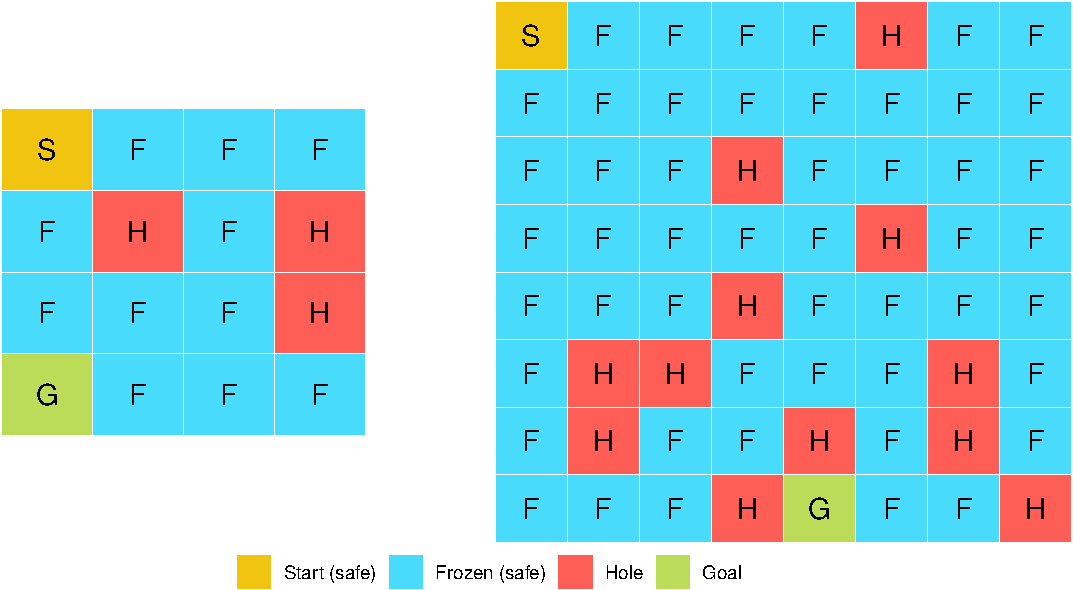
\includegraphics[width=0.7\linewidth]{project_files/figure-latex/lake-1} \end{center}

\begin{verbatim}
##  [1] S F F F F H F H F F F H G F F F
## Levels: S < F < H < G
##  [1] S F F F F H F H F F F H G F F F
## Levels: S < F < H < G
##  [1] S F F F F H F H F F F H G F F F
## Levels: S < F < H < G
##  [1] S F F F F H F H F F F H G F F F
## Levels: S < F < H < G
##  [1] S F F F F H F F F F F F F F F F F F F H F F F F F F F F F H F F F F F
## [36] H F F F F F H H F F F H F F H F F H F H F F F F H G F F H
## Levels: S < F < H < G
##  [1] S F F F F H F F F F F F F F F F F F F H F F F F F F F F F H F F F F F
## [36] H F F F F F H H F F F H F F H F F H F H F F F F H G F F H
## Levels: S < F < H < G
\end{verbatim}

\begin{center}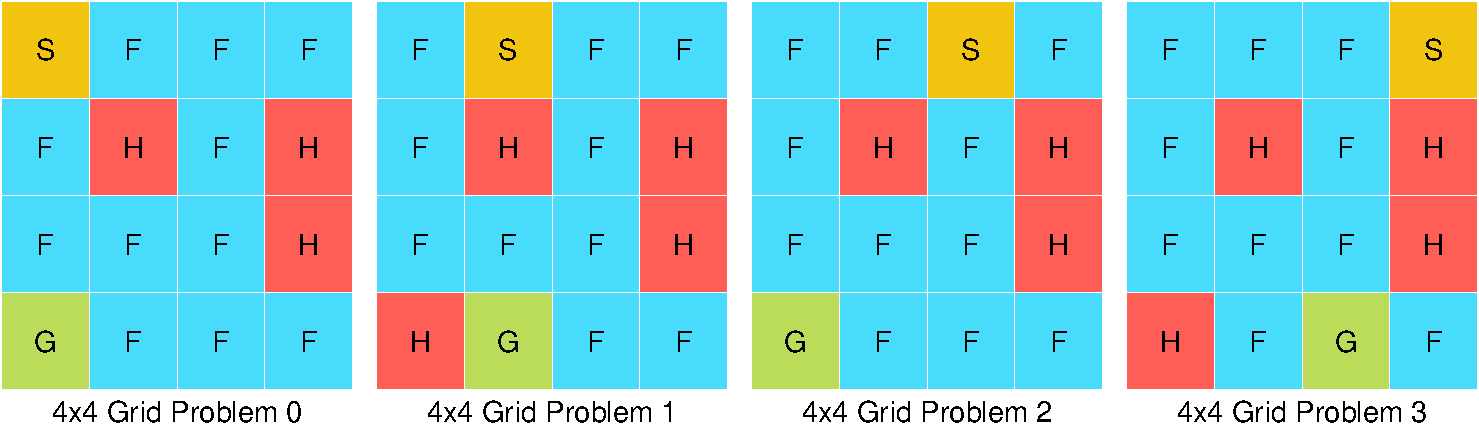
\includegraphics[width=0.9\linewidth]{project_files/figure-latex/lakes-1} \end{center}

\begin{verbatim}
##  [1] S F F F F H F H F F F H G F F F
## Levels: S < F < H < G
##  [1] S F F F F H F H F F F H G F F F
## Levels: S < F < H < G
##  [1] F S F F F H F H F F F H H G F F
## Levels: S < F < H < G
##  [1] F S F F F H F H F F F H H G F F
## Levels: S < F < H < G
##  [1] F F S F F H F H F F F H G F F F
## Levels: S < F < H < G
##  [1] F F S F F H F H F F F H G F F F
## Levels: S < F < H < G
##  [1] F F F S F H F H F F F H H F G F
## Levels: S < F < H < G
##  [1] F F F S F H F H F F F H H F G F
## Levels: S < F < H < G
\end{verbatim}

\begin{center}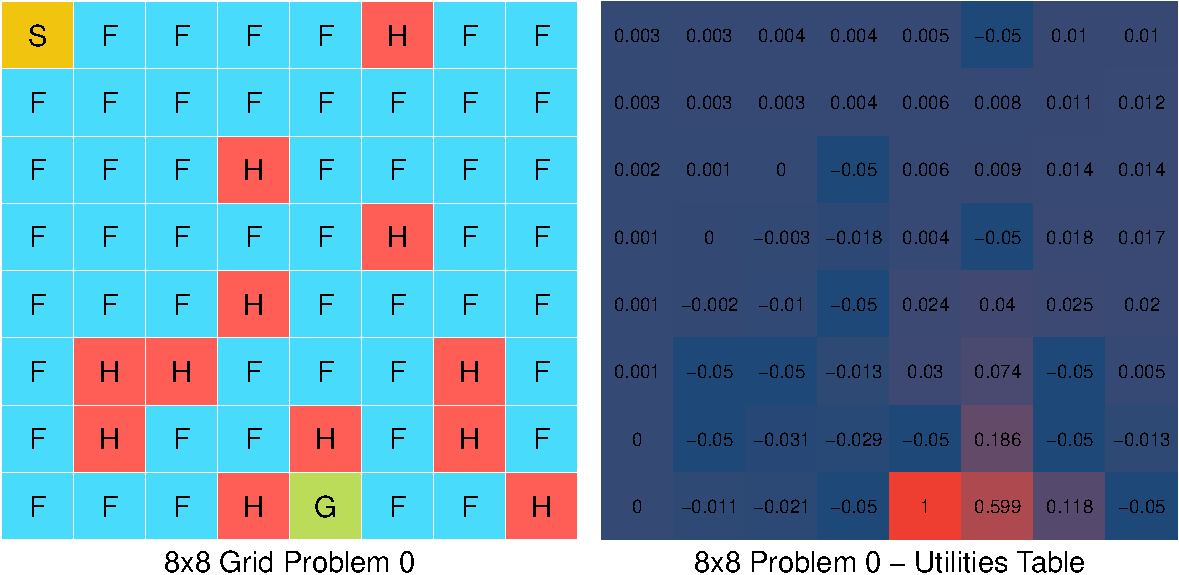
\includegraphics[width=0.9\linewidth]{project_files/figure-latex/lakes3-1} \end{center}

\begin{verbatim}
##  [1] S F F F F H F F F F F F F F F F F F F H F F F F F F F F F H F F F F F
## [36] H F F F F F H H F F F H F F H F F H F H F F F F H G F F H
## Levels: S < F < H < G
##  [1] S F F F F H F F F F F F F F F F F F F H F F F F F F F F F H F F F F F
## [36] H F F F F F H H F F F H F F H F F H F H F F F F H G F F H
## Levels: S < F < H < G
##  [1] H S F F F H F F F F F F F F F F F F F H F F F F F F F F F H F F F F F
## [36] H F F F F F H H F F F H F F H F F H F H F F F F H F G F H
## Levels: S < F < H < G
##  [1] H S F F F H F F F F F F F F F F F F F H F F F F F F F F F H F F F F F
## [36] H F F F F F H H F F F H F F H F F H F H F F F F H F G F H
## Levels: S < F < H < G
\end{verbatim}

\begin{center}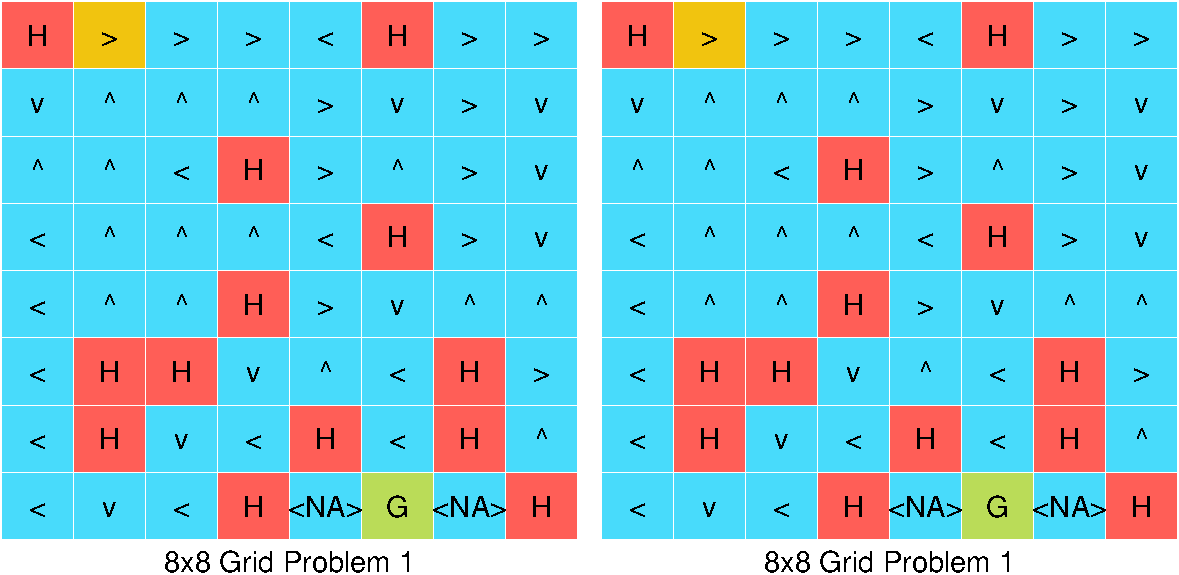
\includegraphics[width=0.9\linewidth]{project_files/figure-latex/lakes3-2} \end{center}

\begin{verbatim}
##  [1] S F F F F H F F F F F F F F F F F F F H F F F F F F F F F H F F F F F
## [36] H F F F F F H H F F F H F F H F F H F H F F F F H G F F H
## Levels: S < F < H < G
##  [1] S F F F F H F F F F F F F F F F F F F H F F F F F F F F F H F F F F F
## [36] H F F F F F H H F F F H F F H F F H F H F F F F H G F F H
## Levels: S < F < H < G
##  [1] H S F F F H F F F F F F F F F F F F F H F F F F F F F F F H F F F F F
## [36] H F F F F F H H F F F H F F H F F H F H F F F F H F G F H
## Levels: S < F < H < G
##  [1] H S F F F H F F F F F F F F F F F F F H F F F F F F F F F H F F F F F
## [36] H F F F F F H H F F F H F F H F F H F H F F F F H F G F H
## Levels: S < F < H < G
\end{verbatim}

\section{Introduction}\label{introduction}

The Loch Lomond Frozen Lake environment is a customized Open AI Gym
derived from FrozenLake (\url{https://gym.openai.com/envs/\#toy_text}).

The goal of this report is to design, implement and evaluate three
diferent virtual agents which are able to navigate across the Loch
Lomond Frozen Lake grid and retrieve the frisbee disc. Three different
agents are analyzed: a senseless agent, a simple agent and a
reinforcement agent.

\section{Agents}\label{agents}

\subsection{Senseless Agent}\label{senseless-agent}

\subsubsection{Evaluation}\label{evaluation}

\subsection{Simple Agent}\label{simple-agent}

\subsubsection{Evaluation}\label{evaluation-1}

\subsection{Reinforcement Learning
Agent}\label{reinforcement-learning-agent}

\subsubsection{Evaluation}\label{evaluation-2}

\section{Conclusions}\label{sec:con}


\end{document}
